% =============================================================================
% Common Distributions
% =============================================================================

\chapter{Common Distributions}
\label{chap:distributions}

This appendix provides a comprehensive reference for probability distributions commonly encountered in statistics and data science. For each distribution, we present the definition, key functions (PMF/PDF, CDF, MGF), moments, and relationships to other distributions.

% =============================================================================
% PART I: DISCRETE DISTRIBUTIONS
% =============================================================================

\section*{Part I: Discrete Distributions}

Discrete distributions assign probabilities to countable outcomes. The probability mass function (PMF) gives $P(X = k)$ for each possible value $k$ in the support.

% ---------------------------
\section{Bernoulli Distribution}
\label{sec:dist-bernoulli}

\begin{itemize}
    \item \textbf{Definition and Parameters:}
    \begin{itemize}
        \item Definition: Represents an experiment with exactly two possible outcomes, often referred to as ``success'' and ``failure''. It is the simplest discrete distribution.
        \item Parameters:
        \begin{itemize}
            \item $p \in [0,1]$: Probability of success.
        \end{itemize}
        \item Notation: $X \sim \text{Bernoulli}(p)$ or $X \sim \text{Bern}(p)$
        \item Support: $\{0, 1\}$
    \end{itemize}

    \item \textbf{Probability Mass Function (PMF):}
    \begin{equation*}
        P(X=k) = p^k (1-p)^{1-k} =
        \begin{cases}
            p & \text{if } k = 1 \\
            1-p & \text{if } k = 0
        \end{cases}
    \end{equation*}

    \item \textbf{Cumulative Distribution Function (CDF):}
    \begin{equation*}
        F(k) = P(X \leq k) =
        \begin{cases}
            0 & \text{for } k < 0 \\
            1-p & \text{for } 0 \leq k < 1 \\
            1 & \text{for } k \geq 1
        \end{cases}
    \end{equation*}

    \item \textbf{Moment Generating Function (MGF):}
    \begin{equation*}
        M_X(t) = E[e^{tX}] = (1-p) + pe^t = 1 - p + pe^t
    \end{equation*}
    This follows directly from the definition: $M_X(t) = e^{t \cdot 0}(1-p) + e^{t \cdot 1}p$.

    \item \textbf{Expected Value and Variance:}
    \begin{align*}
        E(X) &= p \\
        \Var(X) &= p(1-p)
    \end{align*}
    Note that variance is maximised when $p = 0.5$, giving $\Var(X) = 0.25$.

    \item \textbf{Worked Example:}
    \begin{itemize}
        \item Problem Statement: A coin is biased with probability $p = 0.7$ of landing heads. What is the probability it lands tails?
        \item Solution: Using the Bernoulli PMF, $P(X=0) = 1-0.7 = 0.3$.
    \end{itemize}

    \item \textbf{Relation to Other Distributions:}
    \begin{itemize}
        \item A Bernoulli distribution is a special case of the Binomial distribution with $n = 1$.
        \item The sum of $n$ i.i.d.\ Bernoulli$(p)$ random variables follows a Binomial$(n, p)$ distribution.
    \end{itemize}

    \item \textbf{Use Cases:}
    \begin{itemize}
        \item Modelling the outcome of a single trial in any scenario with two possible outcomes: coin tosses, yes/no questions, pass/fail tests, click/no-click events.
    \end{itemize}

    \item \textbf{Miscellaneous Notes:}
    \begin{itemize}
        \item Named after Jacob Bernoulli, a Swiss mathematician.
        \item The Bernoulli distribution is the building block for many other distributions.
    \end{itemize}
\end{itemize}

% ---------------------------
\section{Binomial Distribution}
\label{sec:dist-binomial}

\begin{itemize}
    \item \textbf{Definition and Parameters:}
    \begin{itemize}
        \item Definition: Represents the number of successes in $n$ independent Bernoulli trials, each with the same probability $p$ of success.
        \item Parameters:
        \begin{itemize}
            \item $n \in \{1, 2, 3, \ldots\}$: Number of trials.
            \item $p \in [0,1]$: Probability of success on a single trial.
        \end{itemize}
        \item Notation: $X \sim \text{Binomial}(n, p)$ or $X \sim \text{Bin}(n, p)$
        \item Support: $\{0, 1, 2, \ldots, n\}$
    \end{itemize}

    \item \textbf{Probability Mass Function (PMF):}
    \begin{equation*}
        P(X=k) = \binom{n}{k} p^k (1-p)^{n-k}
    \end{equation*}
    where $\binom{n}{k} = \frac{n!}{k!(n-k)!}$ is the binomial coefficient.

    \item \textbf{Cumulative Distribution Function (CDF):}
    \begin{equation*}
        F(k) = P(X \leq k) = \sum_{i=0}^{\lfloor k \rfloor} \binom{n}{i} p^i (1-p)^{n-i}
    \end{equation*}

    \item \textbf{Moment Generating Function (MGF):}
    \begin{equation*}
        M_X(t) = E[e^{tX}] = \left[(1-p) + pe^t\right]^n
    \end{equation*}
    This follows from the fact that the sum of $n$ independent Bernoulli MGFs gives $(1-p+pe^t)^n$.

    \item \textbf{Expected Value and Variance:}
    \begin{align*}
        E(X) &= np \\
        \Var(X) &= np(1-p)
    \end{align*}

    \item \textbf{Worked Example:}
    \begin{itemize}
        \item Problem Statement: A fair coin is tossed 5 times. What is the probability of getting exactly 3 heads?
        \item Solution: Using the Binomial PMF with $n=5$, $p=0.5$, $k=3$:
        \[P(X=3) = \binom{5}{3} \times 0.5^3 \times 0.5^2 = 10 \times 0.125 \times 0.25 = 0.3125\]
    \end{itemize}

    \item \textbf{Relation to Other Distributions:}
    \begin{itemize}
        \item Binomial$(1, p)$ $\equiv$ Bernoulli$(p)$.
        \item As $n \to \infty$ with $np = \lambda$ held constant (i.e., $p \to 0$), the Binomial converges to Poisson$(\lambda)$.
        \item For large $n$, Binomial$(n, p)$ is approximately Normal$(np, np(1-p))$ (by CLT).
    \end{itemize}

    \item \textbf{Use Cases:}
    \begin{itemize}
        \item Number of heads in coin tosses, number of defective items in a batch, number of correct answers on a multiple-choice test (if guessing randomly).
    \end{itemize}

    \item \textbf{Miscellaneous Notes:}
    \begin{itemize}
        \item One of the most widely used probability distributions in statistics.
        \item Assumes trials are independent with constant success probability.
    \end{itemize}
\end{itemize}

% ---------------------------
\section{Multinomial Distribution}
\label{sec:dist-multinomial}

\begin{itemize}
    \item \textbf{Definition and Parameters:}
    \begin{itemize}
        \item Definition: An extension of the binomial distribution to experiments with more than two possible outcomes. It represents the outcomes of $n$ independent trials, each of which can result in one of $k$ possible categories.
        \item Parameters:
        \begin{itemize}
            \item $n$: Total number of trials.
            \item $k$: Number of possible outcomes/categories.
            \item $p_1, p_2, \ldots, p_k$: Probabilities of each outcome, where $\sum_{i=1}^k p_i = 1$.
        \end{itemize}
        \item Notation: $(X_1, \ldots, X_k) \sim \text{Multinomial}(n, p_1, \ldots, p_k)$
        \item Support: $\{(n_1, \ldots, n_k) : n_i \geq 0, \sum_i n_i = n\}$
    \end{itemize}

    \item \textbf{Probability Mass Function (PMF):}
    \begin{equation*}
        P(X_1=n_1, X_2=n_2, \ldots, X_k=n_k) = \frac{n!}{n_1! n_2! \cdots n_k!} p_1^{n_1} p_2^{n_2} \cdots p_k^{n_k}
    \end{equation*}
    subject to $n_1 + n_2 + \cdots + n_k = n$.

    \item \textbf{Moment Generating Function (MGF):}
    \begin{equation*}
        M_{\mathbf{X}}(t_1, \ldots, t_k) = \left(\sum_{i=1}^{k} p_i e^{t_i}\right)^n
    \end{equation*}

    \item \textbf{Expected Value and Variance:}
    \begin{align*}
        E(X_i) &= np_i \\
        \Var(X_i) &= np_i(1-p_i) \\
        \Cov(X_i, X_j) &= -np_i p_j \quad \text{for } i \neq j
    \end{align*}
    Note the negative covariance: if more outcomes fall in category $i$, fewer are available for category $j$.

    \item \textbf{Worked Example:}
    \begin{itemize}
        \item Problem Statement: A die is rolled 10 times. What is the probability of getting exactly 2 ones, 3 twos, and 5 threes (and zero of the other faces)?
        \item Solution: Using the Multinomial PMF:
        \[
        P = \frac{10!}{2! \cdot 3! \cdot 5! \cdot 0! \cdot 0! \cdot 0!} \times \left(\frac{1}{6}\right)^{10} = \frac{2520}{6^{10}} \approx 4.17 \times 10^{-5}
        \]
    \end{itemize}

    \item \textbf{Relation to Other Distributions:}
    \begin{itemize}
        \item Multinomial with $k = 2$ reduces to the Binomial distribution.
        \item Each marginal $X_i \sim \text{Binomial}(n, p_i)$.
    \end{itemize}

    \item \textbf{Use Cases:}
    \begin{itemize}
        \item Modelling outcomes with multiple categories: dice rolls, categorical survey responses, word counts in text analysis.
    \end{itemize}
\end{itemize}

% ---------------------------
\section{Geometric Distribution}
\label{sec:dist-geometric}

\begin{itemize}
    \item \textbf{Definition and Parameters:}
    \begin{itemize}
        \item Definition: Describes the number of Bernoulli trials needed for the first success. It represents the probability that the first success occurs on the $k$th trial.
        \item Parameters:
        \begin{itemize}
            \item $p \in (0,1]$: Probability of success on a single trial.
        \end{itemize}
        \item Notation: $X \sim \text{Geometric}(p)$ or $X \sim \text{Geom}(p)$
        \item Support: $\{1, 2, 3, \ldots\}$ (trials until first success)

        \textit{Alternative parametrisation}: Some texts define support as $\{0, 1, 2, \ldots\}$ (failures before first success). The formulas below use the ``trials until success'' convention.
    \end{itemize}

    \item \textbf{Probability Mass Function (PMF):}
    \begin{equation*}
        P(X=k) = (1-p)^{k-1} p \quad \text{for } k = 1, 2, 3, \ldots
    \end{equation*}

    \item \textbf{Cumulative Distribution Function (CDF):}
    \begin{equation*}
        F(k) = P(X \leq k) = 1 - (1-p)^k
    \end{equation*}

    \item \textbf{Moment Generating Function (MGF):}
    \begin{equation*}
        M_X(t) = \frac{pe^t}{1 - (1-p)e^t} \quad \text{for } t < -\ln(1-p)
    \end{equation*}

    \item \textbf{Expected Value and Variance:}
    \begin{align*}
        E(X) &= \frac{1}{p} \\
        \Var(X) &= \frac{1-p}{p^2}
    \end{align*}

    \item \textbf{Worked Example:}
    \begin{itemize}
        \item Problem Statement: A fair coin is tossed repeatedly. What is the probability that the first head appears on the 3rd toss?
        \item Solution: With $p = 0.5$:
        \[P(X=3) = (1-0.5)^{3-1} \times 0.5 = 0.25 \times 0.5 = 0.125\]
    \end{itemize}

    \item \textbf{Memorylessness Property:}
    The Geometric distribution is the only discrete distribution with the memoryless property:
    \[P(X > s + t \mid X > s) = P(X > t)\]
    ``Given that no success has occurred in the first $s$ trials, the probability of waiting at least $t$ more trials is the same as starting fresh.''

    \item \textbf{Relation to Other Distributions:}
    \begin{itemize}
        \item Geometric$(p)$ is Negative Binomial$(1, p)$-the special case of waiting for exactly one success.
        \item The continuous analogue is the Exponential distribution.
    \end{itemize}

    \item \textbf{Use Cases:}
    \begin{itemize}
        \item Number of trials until first success: coin tosses until first head, sales calls until first sale, login attempts until success.
    \end{itemize}
\end{itemize}

% ---------------------------
\section{Negative Binomial Distribution}
\label{sec:dist-negbinom}

\begin{itemize}
    \item \textbf{Definition and Parameters:}
    \begin{itemize}
        \item Definition: Describes the number of Bernoulli trials needed to achieve $r$ successes. It represents the probability that the $r$th success occurs on the $k$th trial.
        \item Parameters:
        \begin{itemize}
            \item $r \in \{1, 2, 3, \ldots\}$: Number of successes required.
            \item $p \in (0,1]$: Probability of success on a single trial.
        \end{itemize}
        \item Notation: $X \sim \text{NegBin}(r, p)$
        \item Support: $\{r, r+1, r+2, \ldots\}$
    \end{itemize}

    \item \textbf{Probability Mass Function (PMF):}
    \begin{equation*}
        P(X=k) = \binom{k-1}{r-1} p^r (1-p)^{k-r} \quad \text{for } k = r, r+1, r+2, \ldots
    \end{equation*}
    The binomial coefficient $\binom{k-1}{r-1}$ counts the ways to arrange $r-1$ successes among the first $k-1$ trials.

    \item \textbf{Moment Generating Function (MGF):}
    \begin{equation*}
        M_X(t) = \left(\frac{pe^t}{1 - (1-p)e^t}\right)^r \quad \text{for } t < -\ln(1-p)
    \end{equation*}

    \item \textbf{Expected Value and Variance:}
    \begin{align*}
        E(X) &= \frac{r}{p} \\
        \Var(X) &= \frac{r(1-p)}{p^2}
    \end{align*}

    \item \textbf{Worked Example:}
    \begin{itemize}
        \item Problem Statement: A biased coin with $p = 0.4$ of landing heads is tossed repeatedly. What is the probability that the 5th head appears on the 8th toss?
        \item Solution: We need exactly 4 heads in the first 7 tosses, then a head on toss 8:
        \[P(X=8) = \binom{7}{4} \times 0.4^5 \times 0.6^3 = 35 \times 0.01024 \times 0.216 \approx 0.0774\]
    \end{itemize}

    \item \textbf{Relation to Other Distributions:}
    \begin{itemize}
        \item NegBin$(1, p)$ $\equiv$ Geometric$(p)$.
        \item Sum of $r$ i.i.d.\ Geometric$(p)$ random variables is NegBin$(r, p)$.
        \item The continuous analogue is the Gamma distribution.
    \end{itemize}

    \item \textbf{Use Cases:}
    \begin{itemize}
        \item Number of trials to achieve a fixed number of successes, modelling overdispersed count data (where variance exceeds mean, unlike Poisson).
    \end{itemize}
\end{itemize}

% ---------------------------
\section{Hypergeometric Distribution}
\label{sec:dist-hypergeom}

\begin{itemize}
    \item \textbf{Definition and Parameters:}
    \begin{itemize}
        \item Definition: Describes the probability of obtaining exactly $k$ successes when drawing $n$ items \textit{without replacement} from a finite population of size $N$ containing $K$ success items.
        \item Parameters:
        \begin{itemize}
            \item $N$: Total population size.
            \item $K$: Number of success items in the population.
            \item $n$: Number of items drawn (sample size).
        \end{itemize}
        \item Notation: $X \sim \text{Hypergeometric}(N, K, n)$
        \item Support: $\{\max(0, n-N+K), \ldots, \min(n, K)\}$
    \end{itemize}

    \item \textbf{Probability Mass Function (PMF):}
    \begin{equation*}
        P(X=k) = \frac{\binom{K}{k} \binom{N-K}{n-k}}{\binom{N}{n}}
    \end{equation*}

    \textit{Interpretation}: Choose $k$ successes from $K$ available, and $n-k$ failures from $N-K$ available, divided by total ways to choose $n$ from $N$.

    \item \textbf{Moment Generating Function (MGF):}
    The MGF does not have a simple closed form. It can be expressed using hypergeometric functions:
    \begin{equation*}
        M_X(t) = \frac{\binom{N-K}{n}}{\binom{N}{n}} \cdot {}_2F_1\left(-n, -K; N-K-n+1; e^t\right)
    \end{equation*}
    where ${}_2F_1$ is the hypergeometric function.

    \item \textbf{Expected Value and Variance:}
    \begin{align*}
        E(X) &= n\frac{K}{N} \\
        \Var(X) &= n\frac{K}{N}\frac{N-K}{N}\frac{N-n}{N-1}
    \end{align*}

    The factor $\frac{N-n}{N-1}$ is the \textit{finite population correction factor}. It reduces variance because sampling without replacement introduces negative correlation between draws.

    \item \textbf{Worked Example:}
    \begin{itemize}
        \item Problem Statement: From a standard deck of 52 cards, 5 are drawn without replacement. What is the probability that exactly 3 are spades?
        \item Solution: Here $N=52$, $K=13$ (spades), $n=5$, $k=3$:
        \[P(X=3) = \frac{\binom{13}{3} \binom{39}{2}}{\binom{52}{5}} = \frac{286 \times 741}{2598960} \approx 0.0815\]
    \end{itemize}

    \item \textbf{Relation to Other Distributions:}
    \begin{itemize}
        \item When $N \to \infty$ with $K/N = p$ fixed (i.e., sampling with replacement), Hypergeometric$(N, K, n)$ converges to Binomial$(n, p)$.
        \item Fisher's exact test uses the hypergeometric distribution.
    \end{itemize}

    \item \textbf{Use Cases:}
    \begin{itemize}
        \item Sampling without replacement: drawing cards, quality control (selecting items from a batch), capture-recapture methods in ecology.
    \end{itemize}

    \item \textbf{Miscellaneous Notes:}
    \begin{itemize}
        \item The Hypergeometric provides exact probabilities, while Binomial approximates when sampling without replacement from large populations.
        \item Common in biology/genetics for analysing enrichment of gene sets.
    \end{itemize}
\end{itemize}

% ---------------------------
\section{Poisson Distribution}
\label{sec:dist-poisson}

\begin{itemize}
    \item \textbf{Definition and Parameters:}
    \begin{itemize}
        \item Definition: Describes the number of events occurring in a fixed interval of time or space, given that events occur independently at a constant average rate.
        \item Parameters:
        \begin{itemize}
            \item $\lambda > 0$: Average rate (expected number of events in the interval).
        \end{itemize}
        \item Notation: $X \sim \text{Poisson}(\lambda)$ or $X \sim \text{Pois}(\lambda)$
        \item Support: $\{0, 1, 2, \ldots\}$
    \end{itemize}

    \item \textbf{Probability Mass Function (PMF):}
    \begin{equation*}
        P(X=k) = \frac{\lambda^k e^{-\lambda}}{k!}
    \end{equation*}

    \item \textbf{Cumulative Distribution Function (CDF):}
    \begin{equation*}
        F(k) = P(X \leq k) = e^{-\lambda} \sum_{i=0}^{\lfloor k \rfloor} \frac{\lambda^i}{i!} = \frac{\Gamma(\lfloor k+1 \rfloor, \lambda)}{\lfloor k \rfloor!}
    \end{equation*}
    where $\Gamma(s, x)$ is the upper incomplete gamma function.

    \item \textbf{Moment Generating Function (MGF):}
    \begin{equation*}
        M_X(t) = E[e^{tX}] = e^{\lambda(e^t - 1)}
    \end{equation*}

    \textit{Derivation sketch}: $M_X(t) = \sum_{k=0}^{\infty} e^{tk} \frac{\lambda^k e^{-\lambda}}{k!} = e^{-\lambda} \sum_{k=0}^{\infty} \frac{(\lambda e^t)^k}{k!} = e^{-\lambda} e^{\lambda e^t} = e^{\lambda(e^t - 1)}$.

    \item \textbf{Expected Value and Variance:}
    \begin{align*}
        E(X) &= \lambda \\
        \Var(X) &= \lambda
    \end{align*}
    The equality of mean and variance is a defining characteristic of the Poisson distribution (\textit{equidispersion}).

    \item \textbf{Worked Example:}
    \begin{itemize}
        \item Problem Statement: A call centre receives an average of 5 calls per hour. What is the probability of receiving exactly 7 calls in a given hour?
        \item Solution: With $\lambda = 5$:
        \[P(X=7) = \frac{5^7 e^{-5}}{7!} = \frac{78125 \times 0.00674}{5040} \approx 0.1044\]
    \end{itemize}

    \item \textbf{Key Properties:}
    \begin{itemize}
        \item \textbf{Additivity}: If $X \sim \text{Pois}(\lambda_1)$ and $Y \sim \text{Pois}(\lambda_2)$ are independent, then $X + Y \sim \text{Pois}(\lambda_1 + \lambda_2)$.
        \item \textbf{Conditioning}: Given $X + Y = n$, the conditional distribution of $X$ is Binomial.
    \end{itemize}

    \item \textbf{Relation to Other Distributions:}
    \begin{itemize}
        \item Poisson is the limit of Binomial$(n, p)$ as $n \to \infty$, $p \to 0$, with $np = \lambda$.
        \item For large $\lambda$, Poisson$(\lambda) \approx \text{Normal}(\lambda, \lambda)$.
        \item The inter-arrival times between Poisson events follow an Exponential distribution.
    \end{itemize}

    \item \textbf{Use Cases:}
    \begin{itemize}
        \item Count data: phone calls per hour, website hits per day, number of typos per page, radioactive decay events.
    \end{itemize}

    \item \textbf{Miscellaneous Notes:}
    \begin{itemize}
        \item Named after Sim\'{e}on Denis Poisson.
        \item Particularly known for modelling rare events.
        \item If variance exceeds mean, consider Negative Binomial for overdispersed count data.
    \end{itemize}
\end{itemize}

% =============================================================================
% PART II: CONTINUOUS DISTRIBUTIONS
% =============================================================================

\newpage
\section*{Part II: Continuous Distributions}

Continuous distributions assign probabilities to intervals via probability density functions (PDFs). For any specific value $x$, $P(X = x) = 0$; probabilities are obtained by integrating the PDF over intervals.

% ---------------------------
\section{Uniform Distribution (Continuous)}
\label{sec:dist-uniform}

\begin{itemize}
    \item \textbf{Definition and Parameters:}
    \begin{itemize}
        \item Definition: All values in the interval $[a, b]$ are equally likely. The ``maximum entropy'' distribution for a bounded interval.
        \item Parameters:
        \begin{itemize}
            \item $a$: Lower bound.
            \item $b > a$: Upper bound.
        \end{itemize}
        \item Notation: $X \sim \text{Uniform}(a, b)$ or $X \sim U(a, b)$
        \item Support: $[a, b]$
    \end{itemize}

    \item \textbf{Probability Density Function (PDF):}
    \begin{equation*}
        f(x) = \begin{cases}
            \frac{1}{b-a} & \text{if } a \leq x \leq b \\
            0 & \text{otherwise}
        \end{cases}
    \end{equation*}

    \item \textbf{Cumulative Distribution Function (CDF):}
    \begin{equation*}
        F(x) = \begin{cases}
            0 & \text{if } x < a \\
            \frac{x - a}{b - a} & \text{if } a \leq x \leq b \\
            1 & \text{if } x > b
        \end{cases}
    \end{equation*}

    \item \textbf{Moment Generating Function (MGF):}
    \begin{equation*}
        M_X(t) = \begin{cases}
            \frac{e^{tb} - e^{ta}}{t(b-a)} & \text{if } t \neq 0 \\
            1 & \text{if } t = 0
        \end{cases}
    \end{equation*}

    \item \textbf{Expected Value and Variance:}
    \begin{align*}
        E(X) &= \frac{a + b}{2} \\
        \Var(X) &= \frac{(b - a)^2}{12}
    \end{align*}

    \item \textbf{Worked Example:}
    \begin{itemize}
        \item Problem Statement: A random number generator produces values uniformly between 0 and 10. What is $P(3 \leq X \leq 7)$?
        \item Solution: $P(3 \leq X \leq 7) = \frac{7-3}{10-0} = 0.4$.
    \end{itemize}

    \item \textbf{Use Cases:}
    \begin{itemize}
        \item Random number generation, modelling complete uncertainty over a bounded interval, prior distributions in Bayesian analysis.
    \end{itemize}

    \item \textbf{Relation to Other Distributions:}
    \begin{itemize}
        \item $U(0,1)$ is the standard uniform; all other continuous distributions can be generated from it via inverse transform sampling.
    \end{itemize}
\end{itemize}

% ---------------------------
\section{Normal (Gaussian) Distribution}
\label{sec:dist-normal}

\begin{itemize}
    \item \textbf{Definition and Parameters:}
    \begin{itemize}
        \item Definition: The ``bell curve'' distribution, fundamental to statistics due to the Central Limit Theorem. Characterised by its symmetric, unimodal shape.
        \item Parameters:
        \begin{itemize}
            \item $\mu \in \mathbb{R}$: Mean (location parameter).
            \item $\sigma^2 > 0$: Variance (scale parameter); $\sigma$ is the standard deviation.
        \end{itemize}
        \item Notation: $X \sim \mathcal{N}(\mu, \sigma^2)$ or $X \sim \text{Normal}(\mu, \sigma^2)$
        \item Support: $(-\infty, \infty)$
    \end{itemize}

    \item \textbf{Probability Density Function (PDF):}
    \begin{equation*}
        f(x) = \frac{1}{\sigma\sqrt{2\pi}} \exp\left(-\frac{(x-\mu)^2}{2\sigma^2}\right)
    \end{equation*}

    \item \textbf{Cumulative Distribution Function (CDF):}
    \begin{equation*}
        F(x) = \Phi\left(\frac{x - \mu}{\sigma}\right) = \frac{1}{2}\left[1 + \text{erf}\left(\frac{x - \mu}{\sigma\sqrt{2}}\right)\right]
    \end{equation*}
    where $\Phi$ is the standard normal CDF and $\text{erf}$ is the error function. No closed-form expression exists; values are typically obtained from tables or numerical computation.

    \item \textbf{Moment Generating Function (MGF):}
    \begin{equation*}
        M_X(t) = \exp\left(\mu t + \frac{\sigma^2 t^2}{2}\right)
    \end{equation*}

    \item \textbf{Expected Value and Variance:}
    \begin{align*}
        E(X) &= \mu \\
        \Var(X) &= \sigma^2
    \end{align*}

    \item \textbf{Standard Normal Distribution:}
    When $\mu = 0$ and $\sigma^2 = 1$, we have the \textit{standard normal} $Z \sim \mathcal{N}(0, 1)$:
    \begin{equation*}
        \phi(z) = \frac{1}{\sqrt{2\pi}} e^{-z^2/2}
    \end{equation*}

    \textbf{Standardisation}: Any normal variable can be standardised:
    \begin{equation*}
        Z = \frac{X - \mu}{\sigma} \sim \mathcal{N}(0, 1)
    \end{equation*}

    \item \textbf{Key Properties:}
    \begin{itemize}
        \item \textbf{68-95-99.7 Rule}: Approximately 68\%, 95\%, and 99.7\% of values lie within 1, 2, and 3 standard deviations of the mean.
        \item \textbf{Linear combinations}: If $X \sim \mathcal{N}(\mu, \sigma^2)$, then $aX + b \sim \mathcal{N}(a\mu + b, a^2\sigma^2)$.
        \item \textbf{Sum of normals}: If $X_i \sim \mathcal{N}(\mu_i, \sigma_i^2)$ are independent, then $\sum X_i \sim \mathcal{N}(\sum \mu_i, \sum \sigma_i^2)$.
    \end{itemize}

    \item \textbf{Worked Example:}
    \begin{itemize}
        \item Problem Statement: Heights are normally distributed with mean 170 cm and standard deviation 10 cm. What proportion of people are taller than 185 cm?
        \item Solution: Standardise: $Z = \frac{185 - 170}{10} = 1.5$. Then $P(X > 185) = P(Z > 1.5) = 1 - \Phi(1.5) \approx 1 - 0.9332 = 0.0668$, or about 6.7\%.
    \end{itemize}

    \item \textbf{Relation to Other Distributions:}
    \begin{itemize}
        \item \textbf{Central Limit Theorem}: The sum (or mean) of many i.i.d.\ random variables converges to Normal.
        \item $Z^2 \sim \chi^2_1$ (chi-squared with 1 degree of freedom).
        \item Ratio of independent standard normals follows a Cauchy distribution.
        \item Log-normal: If $X \sim \mathcal{N}(\mu, \sigma^2)$, then $e^X \sim \text{LogNormal}(\mu, \sigma^2)$.
    \end{itemize}

    \item \textbf{Use Cases:}
    \begin{itemize}
        \item Modelling measurement errors, natural phenomena (heights, test scores), financial returns (approximately), inference and hypothesis testing.
    \end{itemize}
\end{itemize}

% ---------------------------
\section{Exponential Distribution}
\label{sec:dist-exponential}

\begin{itemize}
    \item \textbf{Definition and Parameters:}
    \begin{itemize}
        \item Definition: Models the time between events in a Poisson process, or equivalently, the waiting time until the first event. The continuous analogue of the Geometric distribution.
        \item Parameters:
        \begin{itemize}
            \item $\lambda > 0$: Rate parameter (events per unit time).
        \end{itemize}
        \item Notation: $X \sim \text{Exponential}(\lambda)$ or $X \sim \text{Exp}(\lambda)$
        \item Support: $[0, \infty)$

        \textit{Alternative parametrisation}: Some texts use $\beta = 1/\lambda$ (mean/scale parameter).
    \end{itemize}

    \item \textbf{Probability Density Function (PDF):}
    \begin{equation*}
        f(x) = \lambda e^{-\lambda x} \quad \text{for } x \geq 0
    \end{equation*}

    \item \textbf{Cumulative Distribution Function (CDF):}
    \begin{equation*}
        F(x) = 1 - e^{-\lambda x} \quad \text{for } x \geq 0
    \end{equation*}

    \item \textbf{Moment Generating Function (MGF):}
    \begin{equation*}
        M_X(t) = \frac{\lambda}{\lambda - t} \quad \text{for } t < \lambda
    \end{equation*}

    \item \textbf{Expected Value and Variance:}
    \begin{align*}
        E(X) &= \frac{1}{\lambda} \\
        \Var(X) &= \frac{1}{\lambda^2}
    \end{align*}

    \item \textbf{Memorylessness Property:}
    The Exponential distribution is the only continuous distribution with the memoryless property:
    \begin{equation*}
        P(X > s + t \mid X > s) = P(X > t)
    \end{equation*}
    ``Given that no event has occurred by time $s$, the probability of waiting at least $t$ more units is the same as starting fresh.''

    \item \textbf{Worked Example:}
    \begin{itemize}
        \item Problem Statement: Light bulbs fail at a rate of 0.1 per year (exponentially distributed). What is the probability a bulb lasts more than 15 years?
        \item Solution: $P(X > 15) = e^{-0.1 \times 15} = e^{-1.5} \approx 0.223$.
    \end{itemize}

    \item \textbf{Relation to Other Distributions:}
    \begin{itemize}
        \item Exponential$(\lambda)$ is Gamma$(1, \lambda)$-a gamma with shape parameter 1.
        \item Sum of $n$ i.i.d.\ Exponential$(\lambda)$ is Gamma$(n, \lambda)$.
        \item Inter-arrival times in a Poisson$(\lambda)$ process are Exponential$(\lambda)$.
        \item Continuous analogue of Geometric distribution.
    \end{itemize}

    \item \textbf{Use Cases:}
    \begin{itemize}
        \item Waiting times: time until next customer arrival, time until equipment failure (constant hazard rate), radioactive decay.
    \end{itemize}
\end{itemize}

% ---------------------------
\section{Gamma Distribution}
\label{sec:dist-gamma}

\begin{itemize}
    \item \textbf{Definition and Parameters:}
    \begin{itemize}
        \item Definition: A flexible family of distributions for positive continuous variables. Models the time until $\alpha$ events occur in a Poisson process (generalisation of Exponential).
        \item Parameters:
        \begin{itemize}
            \item $\alpha > 0$: Shape parameter (number of events).
            \item $\beta > 0$: Rate parameter (events per unit time).
        \end{itemize}
        \item Notation: $X \sim \text{Gamma}(\alpha, \beta)$
        \item Support: $(0, \infty)$

        \textit{Alternative parametrisation}: Some texts use scale $\theta = 1/\beta$ instead of rate $\beta$.
    \end{itemize}

    \item \textbf{Probability Density Function (PDF):}
    \begin{equation*}
        f(x) = \frac{\beta^\alpha}{\Gamma(\alpha)} x^{\alpha-1} e^{-\beta x} \quad \text{for } x > 0
    \end{equation*}
    where $\Gamma(\alpha) = \int_0^\infty t^{\alpha-1} e^{-t} \, dt$ is the gamma function. For positive integers, $\Gamma(n) = (n-1)!$.

    \item \textbf{Cumulative Distribution Function (CDF):}
    \begin{equation*}
        F(x) = \frac{\gamma(\alpha, \beta x)}{\Gamma(\alpha)}
    \end{equation*}
    where $\gamma(\alpha, x)$ is the lower incomplete gamma function.

    \item \textbf{Moment Generating Function (MGF):}
    \begin{equation*}
        M_X(t) = \left(\frac{\beta}{\beta - t}\right)^\alpha \quad \text{for } t < \beta
    \end{equation*}

    \item \textbf{Expected Value and Variance:}
    \begin{align*}
        E(X) &= \frac{\alpha}{\beta} \\
        \Var(X) &= \frac{\alpha}{\beta^2}
    \end{align*}

    \item \textbf{Special Cases:}
    \begin{itemize}
        \item Gamma$(1, \beta)$ = Exponential$(\beta)$
        \item Gamma$(n/2, 1/2)$ = $\chi^2_n$ (chi-squared with $n$ degrees of freedom)
        \item Gamma$(\alpha, \alpha)$ has mean 1 for any $\alpha$
    \end{itemize}

    \item \textbf{Worked Example:}
    \begin{itemize}
        \item Problem Statement: Calls arrive at a rate of 2 per minute. What is the expected time until the 5th call, and its variance?
        \item Solution: Time until 5th call is Gamma$(5, 2)$. Mean $= 5/2 = 2.5$ minutes, Variance $= 5/4 = 1.25$ minutes$^2$.
    \end{itemize}

    \item \textbf{Relation to Other Distributions:}
    \begin{itemize}
        \item Sum of $n$ i.i.d.\ Exponential$(\beta)$ is Gamma$(n, \beta)$.
        \item Continuous analogue of Negative Binomial.
        \item Chi-squared is a special case.
        \item Gamma is conjugate prior for Poisson rate parameter in Bayesian inference.
    \end{itemize}

    \item \textbf{Use Cases:}
    \begin{itemize}
        \item Waiting times for multiple events, modelling positive skewed data (insurance claims, rainfall), Bayesian inference.
    \end{itemize}
\end{itemize}

% ---------------------------
\section{Beta Distribution}
\label{sec:dist-beta}

\begin{itemize}
    \item \textbf{Definition and Parameters:}
    \begin{itemize}
        \item Definition: A flexible family of distributions on the interval $[0, 1]$. Commonly used to model probabilities, proportions, and percentages.
        \item Parameters:
        \begin{itemize}
            \item $\alpha > 0$: Shape parameter (can be interpreted as ``pseudo-counts'' of successes + 1).
            \item $\beta > 0$: Shape parameter (can be interpreted as ``pseudo-counts'' of failures + 1).
        \end{itemize}
        \item Notation: $X \sim \text{Beta}(\alpha, \beta)$
        \item Support: $(0, 1)$ or $[0, 1]$ depending on parameter values
    \end{itemize}

    \item \textbf{Probability Density Function (PDF):}
    \begin{equation*}
        f(x) = \frac{x^{\alpha-1}(1-x)^{\beta-1}}{B(\alpha, \beta)} \quad \text{for } 0 < x < 1
    \end{equation*}
    where $B(\alpha, \beta) = \frac{\Gamma(\alpha)\Gamma(\beta)}{\Gamma(\alpha+\beta)}$ is the beta function.

    \item \textbf{Cumulative Distribution Function (CDF):}
    \begin{equation*}
        F(x) = I_x(\alpha, \beta) = \frac{B(x; \alpha, \beta)}{B(\alpha, \beta)}
    \end{equation*}
    where $I_x$ is the regularised incomplete beta function.

    \item \textbf{Moment Generating Function (MGF):}
    \begin{equation*}
        M_X(t) = 1 + \sum_{k=1}^{\infty} \left(\prod_{r=0}^{k-1} \frac{\alpha + r}{\alpha + \beta + r}\right) \frac{t^k}{k!}
    \end{equation*}
    The MGF does not have a simple closed form; it can be expressed in terms of confluent hypergeometric functions.

    \item \textbf{Expected Value and Variance:}
    \begin{align*}
        E(X) &= \frac{\alpha}{\alpha + \beta} \\
        \Var(X) &= \frac{\alpha\beta}{(\alpha + \beta)^2(\alpha + \beta + 1)}
    \end{align*}

    \item \textbf{Special Cases and Shape Behaviour:}
    \begin{itemize}
        \item Beta$(1, 1)$ = Uniform$(0, 1)$
        \item Beta$(\alpha, \alpha)$ is symmetric around 0.5
        \item $\alpha < 1, \beta < 1$: U-shaped (bimodal at boundaries)
        \item $\alpha > 1, \beta > 1$: Unimodal
        \item $\alpha = \beta = 0.5$: Arcsine distribution
    \end{itemize}

    \item \textbf{Worked Example:}
    \begin{itemize}
        \item Problem Statement: In Bayesian inference, you start with a Beta$(2, 2)$ prior on a coin's probability of heads. After observing 7 heads and 3 tails, what is the posterior distribution?
        \item Solution: The posterior is Beta$(2 + 7, 2 + 3)$ = Beta$(9, 5)$, with posterior mean $9/14 \approx 0.643$.
    \end{itemize}

    \item \textbf{Relation to Other Distributions:}
    \begin{itemize}
        \item Conjugate prior for the Binomial/Bernoulli probability parameter.
        \item If $X \sim \text{Gamma}(\alpha, 1)$ and $Y \sim \text{Gamma}(\beta, 1)$ are independent, then $\frac{X}{X+Y} \sim \text{Beta}(\alpha, \beta)$.
        \item Order statistics of Uniform$(0,1)$ follow Beta distributions.
    \end{itemize}

    \item \textbf{Use Cases:}
    \begin{itemize}
        \item Modelling probabilities and proportions, Bayesian inference (prior for binomial $p$), A/B testing, project completion percentages.
    \end{itemize}
\end{itemize}

% =============================================================================
% PART III: DISTRIBUTION RELATIONSHIPS
% =============================================================================

\newpage
\section*{Part III: Distribution Relationships and Summary}

Understanding how distributions relate to each other provides insight into when approximations are valid and reveals the underlying structure of probability theory.

\subsection*{Relationship Diagram}

The following diagram illustrates key relationships between distributions:

\begin{center}
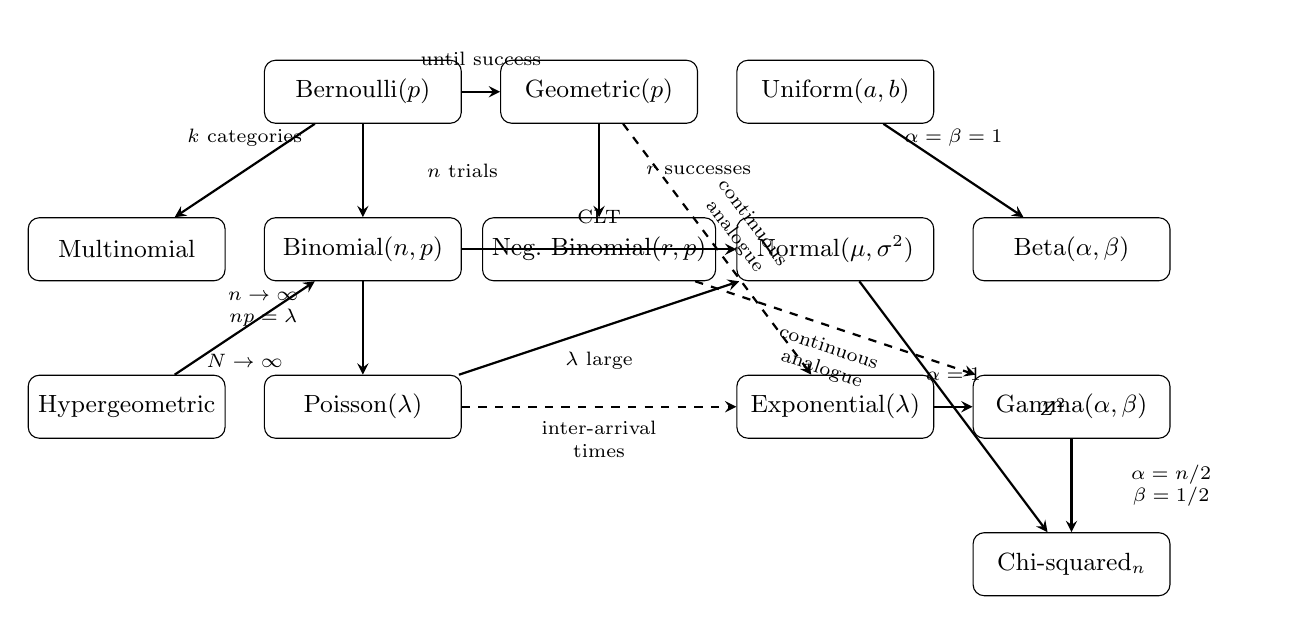
\begin{tikzpicture}[
    node distance=2cm,
    every node/.style={draw, rounded corners, minimum width=2.5cm, minimum height=0.8cm, align=center, font=\small},
    arrow/.style={->, >=stealth, thick},
    label/.style={font=\scriptsize, draw=none, fill=none}
]

% Discrete distributions (left side)
\node (bern) at (0, 6) {Bernoulli$(p)$};
\node (binom) at (0, 4) {Binomial$(n,p)$};
\node (multinom) at (-3, 4) {Multinomial};
\node (geom) at (3, 6) {Geometric$(p)$};
\node (negbin) at (3, 4) {Neg.\ Binomial$(r,p)$};
\node (hypergeom) at (-3, 2) {Hypergeometric};
\node (poisson) at (0, 2) {Poisson$(\lambda)$};

% Continuous distributions (right side / bottom)
\node (uniform) at (6, 6) {Uniform$(a,b)$};
\node (normal) at (6, 4) {Normal$(\mu,\sigma^2)$};
\node (exp) at (6, 2) {Exponential$(\lambda)$};
\node (gamma) at (9, 2) {Gamma$(\alpha,\beta)$};
\node (beta) at (9, 4) {Beta$(\alpha,\beta)$};
\node (chisq) at (9, 0) {Chi-squared$_n$};

% Arrows with labels
\draw[arrow] (bern) -- node[label, right] {$n$ trials} (binom);
\draw[arrow] (bern) -- node[label, above] {$k$ categories} (multinom);
\draw[arrow] (bern) -- node[label, above] {until success} (geom);
\draw[arrow] (geom) -- node[label, right] {$r$ successes} (negbin);
\draw[arrow] (binom) -- node[label, left, pos=0.3] {$n\to\infty$\\$np=\lambda$} (poisson);
\draw[arrow] (hypergeom) -- node[label, below] {$N\to\infty$} (binom);
\draw[arrow] (binom) -- node[label, above] {CLT} (normal);
\draw[arrow] (poisson) -- node[label, below] {$\lambda$ large} (normal);

% Continuous relationships
\draw[arrow] (exp) -- node[label, above] {$\alpha=1$} (gamma);
\draw[arrow] (gamma) -- node[label, right] {$\alpha=n/2$\\$\beta=1/2$} (chisq);
\draw[arrow] (normal) -- node[label, right] {$Z^2$} (chisq);
\draw[arrow] (uniform) -- node[label, above] {$\alpha=\beta=1$} (beta);

% Discrete-continuous connections
\draw[arrow, dashed] (geom) -- node[label, above, sloped] {continuous\\analogue} (exp);
\draw[arrow, dashed] (negbin) -- node[label, below, sloped] {continuous\\analogue} (gamma);
\draw[arrow, dashed] (poisson) -- node[label, below, sloped] {inter-arrival\\times} (exp);

\end{tikzpicture}
\end{center}

\textit{Solid arrows} indicate limiting relationships or special cases. \textit{Dashed arrows} indicate analogous relationships between discrete and continuous distributions.

\subsection*{Summary Table: Discrete Distributions}

\begin{center}
\renewcommand{\arraystretch}{1.4}
\begin{tabular}{lcccc}
\toprule
\textbf{Distribution} & \textbf{PMF} & \textbf{Mean} & \textbf{Variance} & \textbf{MGF} \\
\midrule
Bernoulli$(p)$ & $p^k(1-p)^{1-k}$ & $p$ & $p(1-p)$ & $1-p+pe^t$ \\
Binomial$(n,p)$ & $\binom{n}{k}p^k(1-p)^{n-k}$ & $np$ & $np(1-p)$ & $(1-p+pe^t)^n$ \\
Geometric$(p)$ & $(1-p)^{k-1}p$ & $\frac{1}{p}$ & $\frac{1-p}{p^2}$ & $\frac{pe^t}{1-(1-p)e^t}$ \\
Neg.\ Binomial$(r,p)$ & $\binom{k-1}{r-1}p^r(1-p)^{k-r}$ & $\frac{r}{p}$ & $\frac{r(1-p)}{p^2}$ & $\left(\frac{pe^t}{1-(1-p)e^t}\right)^r$ \\
Poisson$(\lambda)$ & $\frac{\lambda^k e^{-\lambda}}{k!}$ & $\lambda$ & $\lambda$ & $e^{\lambda(e^t-1)}$ \\
\bottomrule
\end{tabular}
\end{center}

\subsection*{Summary Table: Continuous Distributions}

\begin{center}
\renewcommand{\arraystretch}{1.4}
\begin{tabular}{lcccc}
\toprule
\textbf{Distribution} & \textbf{PDF} & \textbf{Mean} & \textbf{Variance} & \textbf{MGF} \\
\midrule
Uniform$(a,b)$ & $\frac{1}{b-a}$ & $\frac{a+b}{2}$ & $\frac{(b-a)^2}{12}$ & $\frac{e^{tb}-e^{ta}}{t(b-a)}$ \\
Normal$(\mu,\sigma^2)$ & $\frac{1}{\sigma\sqrt{2\pi}}e^{-\frac{(x-\mu)^2}{2\sigma^2}}$ & $\mu$ & $\sigma^2$ & $e^{\mu t + \frac{\sigma^2 t^2}{2}}$ \\
Exponential$(\lambda)$ & $\lambda e^{-\lambda x}$ & $\frac{1}{\lambda}$ & $\frac{1}{\lambda^2}$ & $\frac{\lambda}{\lambda - t}$ \\
Gamma$(\alpha,\beta)$ & $\frac{\beta^\alpha}{\Gamma(\alpha)}x^{\alpha-1}e^{-\beta x}$ & $\frac{\alpha}{\beta}$ & $\frac{\alpha}{\beta^2}$ & $\left(\frac{\beta}{\beta-t}\right)^\alpha$ \\
Beta$(\alpha,\beta)$ & $\frac{x^{\alpha-1}(1-x)^{\beta-1}}{B(\alpha,\beta)}$ & $\frac{\alpha}{\alpha+\beta}$ & $\frac{\alpha\beta}{(\alpha+\beta)^2(\alpha+\beta+1)}$ & (complex) \\
\bottomrule
\end{tabular}
\end{center}

\subsection*{Key Relationships and Approximations}

\begin{enumerate}
    \item \textbf{Binomial to Poisson}: When $n$ is large, $p$ is small, and $\lambda = np$ is moderate:
    \[\text{Binomial}(n, p) \approx \text{Poisson}(np)\]
    Rule of thumb: $n \geq 20$ and $p \leq 0.05$.

    \item \textbf{Binomial to Normal} (CLT): When both $np$ and $n(1-p)$ are large (typically $\geq 10$):
    \[\text{Binomial}(n, p) \approx \mathcal{N}(np, np(1-p))\]

    \item \textbf{Poisson to Normal}: When $\lambda$ is large (typically $\geq 30$):
    \[\text{Poisson}(\lambda) \approx \mathcal{N}(\lambda, \lambda)\]

    \item \textbf{Hypergeometric to Binomial}: When $N$ is much larger than $n$ (finite population correction negligible):
    \[\text{Hypergeometric}(N, K, n) \approx \text{Binomial}(n, K/N)\]

    \item \textbf{Conjugate Pairs} (Bayesian inference):
    \begin{itemize}
        \item Beta prior + Binomial likelihood $\to$ Beta posterior
        \item Gamma prior + Poisson likelihood $\to$ Gamma posterior
        \item Normal prior + Normal likelihood $\to$ Normal posterior
    \end{itemize}
\end{enumerate}

\subsection*{Memoryless Distributions}

Only two distributions possess the memoryless property $P(X > s + t \mid X > s) = P(X > t)$:
\begin{itemize}
    \item \textbf{Geometric} (discrete): Number of trials until first success
    \item \textbf{Exponential} (continuous): Waiting time until first event
\end{itemize}

This property implies a ``constant hazard rate''-the probability of an event occurring in the next instant is independent of how long you have already waited.
